\mysubsubsection{Layered depthmap estimation}

\noindent We have used ``ours\_1'' data in~\cite{layered_depthmap} for
the experiments. Figure~\ref{fig:layered_depthmap_convergence} shows
that Fusion Move, Parallel Fusion Move and SF-MF all got stuck in local
minima, which is due to the lack of multi-way fusion.  Layered depthmap
estimation is a challenging problem with very large solution space. The
binary fusion of solution proposals is too restrictive to make any
improvements.  This coincides with the observation in
\cite{layered_depthmap} that binary fusion of proposal solutions is not
as powerful as their subspace fusion which is a special form of
multi-way fusion here. Lastly, solution sharing also plays an important
role for this challenging problem for exactly the same reason, as SF
performs much better than SF-SS.

%
%From the plot, we can see that, Fusion Move, Parallel Fusion Move, and
%SF-MF all stalk at a high energy state.
To further study the effects of multi-way fusion, we have varied the
value of $\alpha$ which controls the number of solution proposals to be
fused in SF-SS model (See
Fig.~\ref{fig:layered_depthmap_by_alpha}). Note that we have used SF-SS
instead of SF to disable solution sharing and better observe the effects
of multi-way fusion.
% SF-SS model (disable solution sharing to
%better observe the effect of multi-way fusion) while keeping other
%parameters the same and plot the energy minimization process in figure
It is interesting to see that more multi-way fusion takes longer to
converge, but finds a lower energy state at the end.

At the end we examined the role of multi-threading by varying the number of threads N in our most general model SF (See Fig.~\ref{fig:layered_depthmap_by_N}).~\footnote{Note that we have the constraint that $\beta \leq N-1$, we always use $\beta = N-1$ in this experiment.}  It is natural that our SF model find lower energy faster with more threads. While due to the inherited randomness in the proposal and fusion scheme of Fusion Move methods, the speed up is not propotional to the number of threads.
%We can see that as the number of
%ways to fuse becomes larger, each fusion step takes longer time, but the
%chance of finding a lower energy state increases.

\begin{figure}[tb]
  \centering
  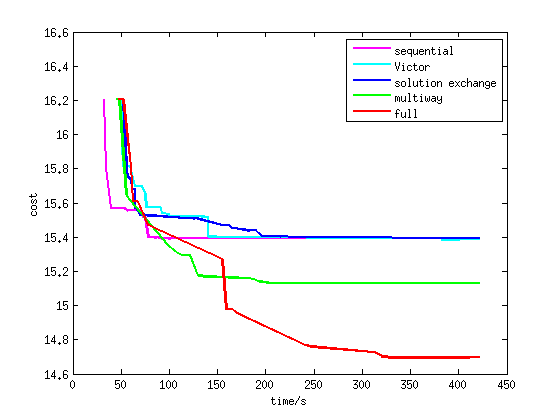
\includegraphics[width=0.8\columnwidth]{figure/layered_depthmap_convergence.png}
  \caption{Energy plots for the layered depthmap estimation
 problem. Both the multi-way fusion and the solution sharing are important
 for this challenging problem.}\label{fig:layered_depthmap_convergence}
\end{figure}

\begin{figure}[tb]
  \centering
  \begin{subfigure}[b]{0.49\columnwidth}
    \centering
    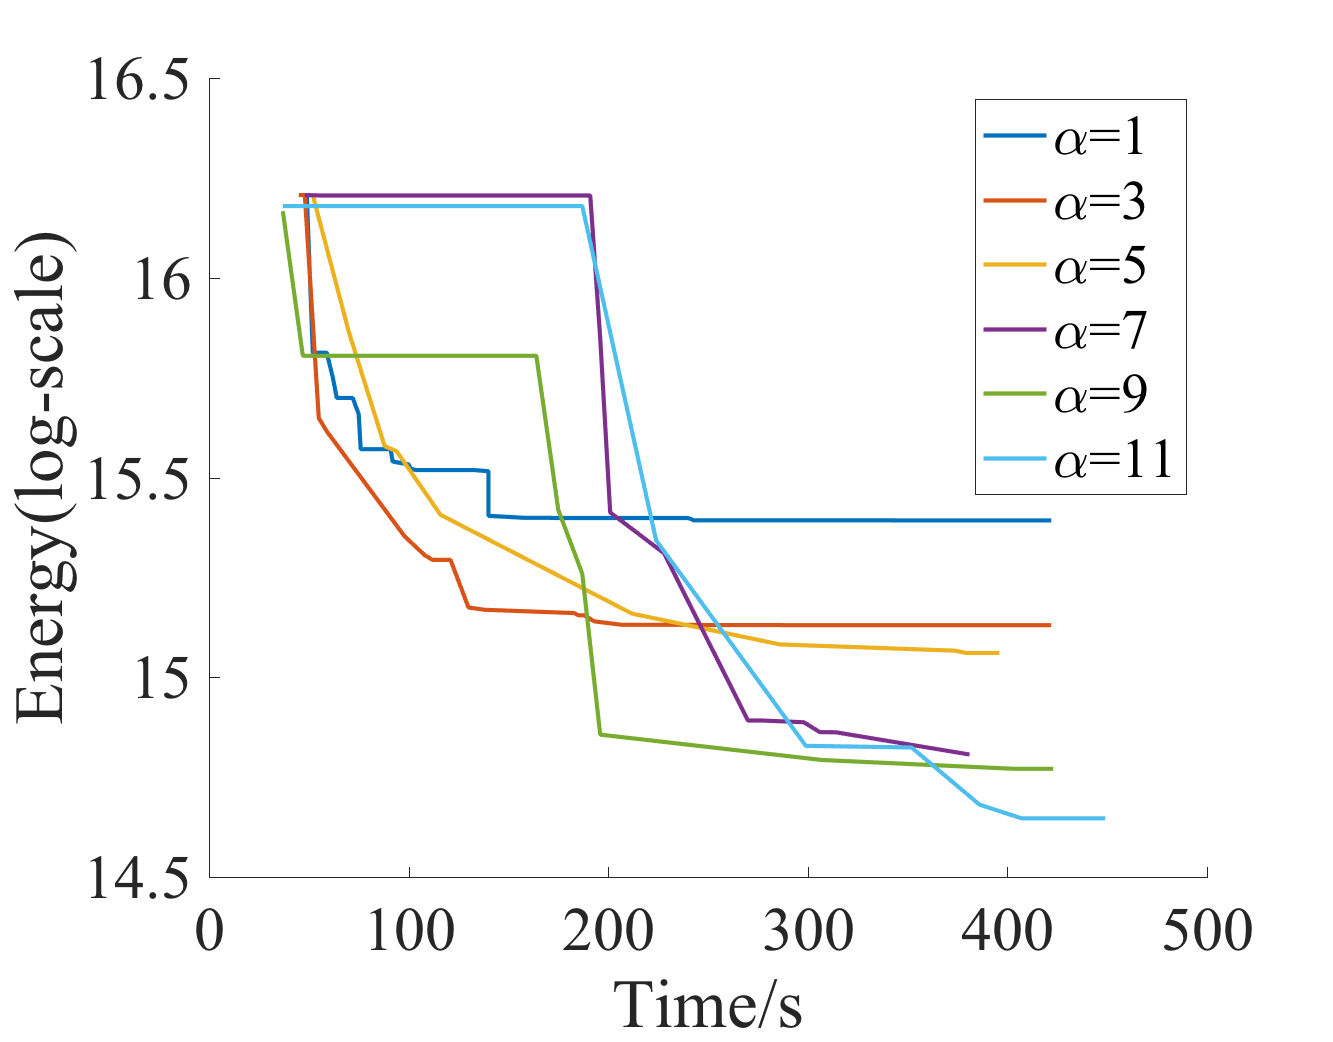
\includegraphics[width=\columnwidth]{figure/layered_depthmap_by_alpha.png}
    \caption{}
    \label{fig:optical_flow_by_alpha}
  \end{subfigure}  
  \begin{subfigure}[b]{0.49\columnwidth}
    \centering
    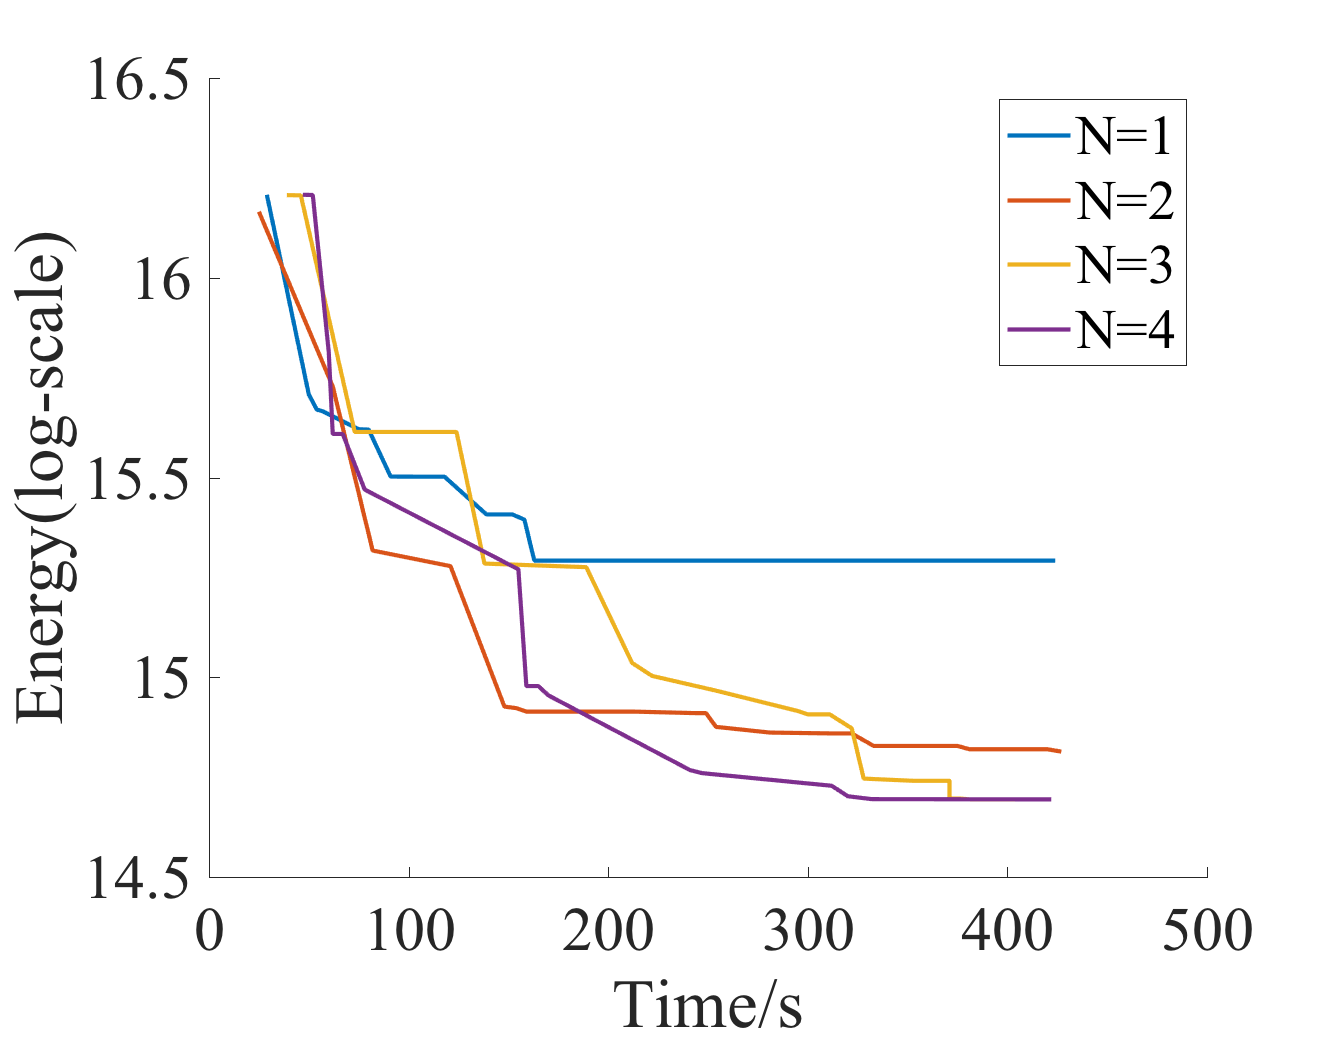
\includegraphics[width=\columnwidth]{figure/layered_depthmap_by_N.png}
    \caption{}
    \label{fig:optical_flow_by_N}
  \end{subfigure}
  \caption{(a) Energy plots for layered depthmap estimation with varying
    $\alpha$. More multi-way fusion takes longer to converge but finds a better   
    solution at the end. (b) Energy plots for layered depthmap estimation with varying number of threads N. More threads find lower energy faster.}
  \label{fig:layered_depthmap_by_alpha_N}
\end{figure}

